
\eucommentary{Please provide the following:\\
\begin{compactitem}
\item
brief presentation of the overall structure of the work plan;
\item
timing of the different work packages and their components (Gantt chart or similar);
\item
detailed work description, i.e.:
\begin{compactitem}
\item
a description of each work package (table 3.1a);
\item
a list of work packages (table 3.1b);
\item
a list of major deliverables (table 3.1c);
\end{compactitem}
\item
graphical presentation of the components showing how they inter-relate (Pert chart or similar).
\end{compactitem}
}

\subsubsection{Quality and efficiency of the implementation}\label{sec:workplan-structure}

\ifgrantagreement The \else As shown in Table~\ref{fig:wplist} and
Figure~\ref{fig:workpackages}, the \fi work plan is broken down into five work
packages: \WPref{reproducibility} focuses on robustness improvements of the
Binder tools, \WPref{impact} is advancing the Binder tools feature set to
increase the impact of the tools and project, \WPref{applications} applies and
evaluates the reproducibility tools in real-world research contexts.
\WPref{education} is focused on engaging with and educating researchers and the
wider public in best practices for reproducible science. This is complemented by
the usual management work package (\WPref{management}).


\TODO{Gantt chart link:
  Remove the next sentence, if we remove the Ganttchart.} The Gantt chart on
Page~\pageref{fig:gantt} illustrates the timeline for the various tasks for
these work packages.
%, including inter-task dependencies.

\ifgrantagreement\else
%\makeatletter\wp@total@RM{management}\makeatother
\wpfigstyle{\footnotesize\def\tabcolsep{3.5pt}}
%\wpfig[pages,type,start,end]
{\wpfig}
\fi

\begin{figure}[htb]
  \centering
  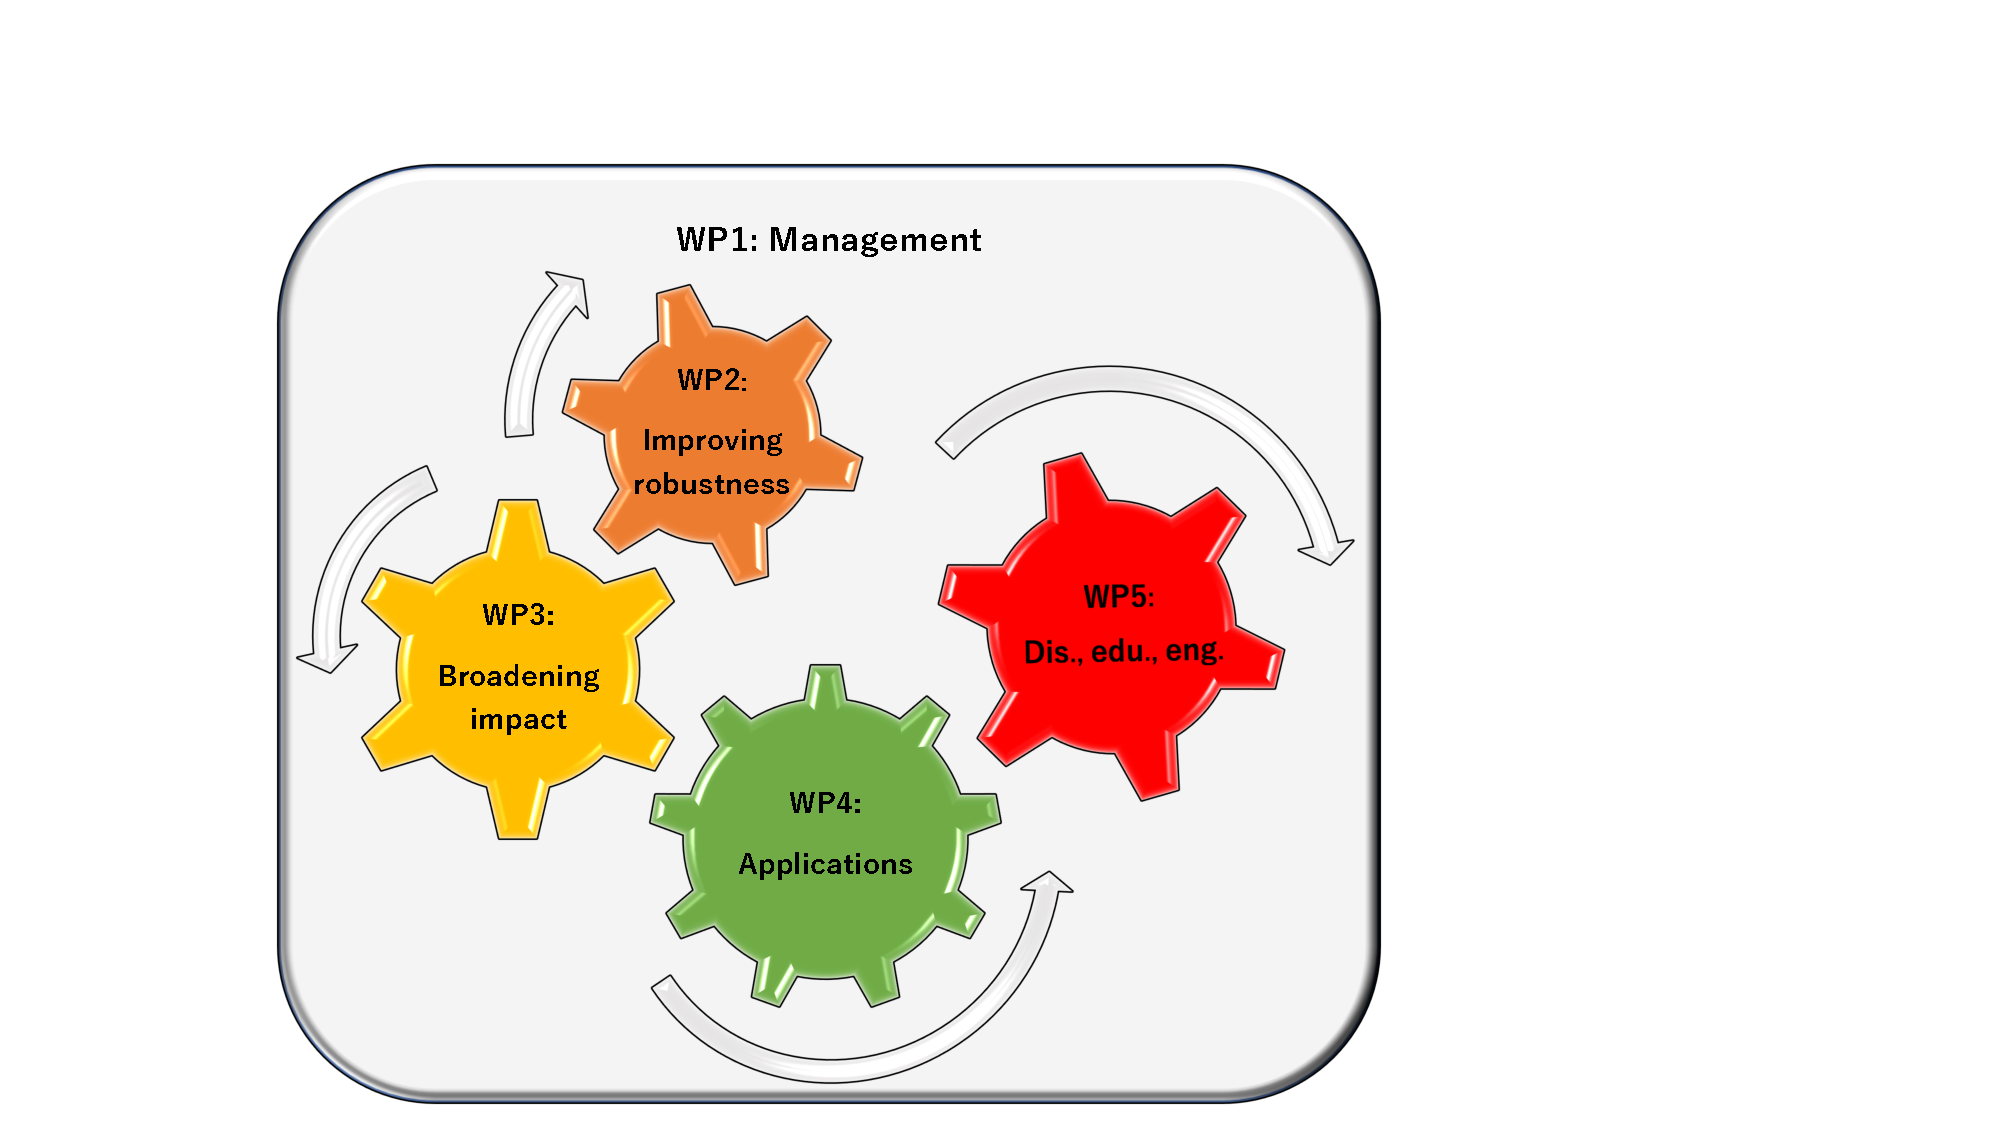
\includegraphics[width=0.7\textwidth]{images/WP.pdf}
  \caption{
    \label{fig:workpackages}
    The relationships and interactions of the work packages,
    broken up into four categories: Management (WP1),
    Development of new functionality surrounding Jupyter's Binder tools to improving robustness 
    and Broadening impact (WP2, WP3),
    Applications of tools developed in real world research context (WP4),
    and Dissemination, education, and engagement (WP5: Dis., edu., eng.).
  }
\end{figure}

% \subsubsection{How the Work Packages will Achieve the Project Objectives}
% \label{sssec:how_the_work_packages_will_achieve}

\ganttchart[draft,xscale=.33,milestones]
\TODO{Gantt chart: HF: seems useless as it is. Can we fiddle with options? Otherwise
remove.}

\ifgrantagreement\else
\newpage
\subsubsection{Deliverables}\label{sec:deliverables}
\inputdelivs{9.3cm}
\TODO{Strage vertical lines at the left of the bottom of table~\ref{sec:deliverables}?}
\fi

% Save space for exploitation
% \newpage
\subsubsection{Milestones}\label{sec:milestones}
\subsubsection{Milestones}\label{sec:milestones}

\eucommentary{Milestones means control points in the project that help to chart progress. Milestones may
correspond to the completion of a key deliverable, allowing the next phase of the work to begin.
They may also be needed at intermediary points so that, if problems have arisen, corrective
measures can be taken. A milestone may be a critical decision point in the project where, for
example, the consortium must decide which of several technologies to adopt for further
development.
}

\begin{draft}
\begin{verbatim}
TODO:
- [x] sort milestones
- [ ] check dates
- [ ] omit descriptions? Template doesn't have any
- [x] involved WP: both input and output, or just input?
\end{verbatim}
\end{draft}

\begin{milestones}
  \milestone[
    id=conda-time,
    month=6,
    wps={reproducibility},
    verif={Feature available in conda/mamba software},
    ]
  {Select conda packages by date}
  {
  The conda/mamba package manager shall be able to
  select packages for installation based on a given date.
  Necessary for repo2docker to best take time into account
  when creating a software environment.
  }

  \milestone[
    id=study,
    month=12,
    wps={reproducibility,education},
    verif={Report produced},
    ]
  {Reproducibility study and evaluation tool}
  {
  We will have preliminary study results and an associated tool,
  regarding the reproducibility of repositories with repo2docker.
  These results will inform future development of the tools in WP2,
  as well as best practices resources and education in WP5.
  }

  \milestone[
    id=rm-docker,
    month=15,
    wps={impact,applications},
    verif={Feature available in repo2docker software},
    ]
  {Support for alternative container technologies in repo2docker for suitability in HPC}
  {
  The Docker container runtime is not suitable in all cases.
  In order to proceed with some demonstrators in WP4,
  we must ensure compatibility with container runtimes supported by our HPC providers,
  such as Singularity.
  }

  \milestone[
    id=prototype,
    month=12,
    wps={applications,impact},
    verif={
      Deployed first functional prototypes of science demonstrators.
      Early users are able to access and test prototype services
    }
    ]
  {Prototype demonstrator services}
  {
  By this point, prototype demonstrator services will be useful and accessible
  to a broad range of users, and we will have begun to experiment with early-adopter
  users and local demonstrators to guide further development in WP3,
  ensuring that development serves the reproducibility needs of the global science community.
  }

  \milestone[
    id=docs-online,
    month=12,
    wps={education},
    verif={Resources available from project website},
    ]
  {Draft best practices documentation}
  {
  Draft version of documentation for best practices is online.
  Required starting point for education tasks in WP5.
  }

  \milestone[
    id=repo2docker-time,
    month=18,
    wps={reproducibility},
    verif={Feature available in repo2docker software},
    ]
  {repo2docker takes publication time into account}
  {
  By taking publication time into account,
  repo2docker will reproduce environments with higher fidelity,
  especially when environments are not fully or strictly specified.
  }

  \milestone[
    id=data-publishing,
    month=18,
    wps={impact,applications},
    verif={Demonstrated example deployment},
    ]
  {Practical support for authenticated data publishing}
  {
  It shall be practical to deploy BinderHub with performant, authenticated access to large datasets,
  required for some advanced science demonstrators in WP4.
  }

  \milestone[
    id=repo2docker-improved,
    month=24,
    wps={reproducibility},
    verif={Delivered in repo2docker software; Repeat study, comparing baseline results form start of project},
    ]
  {repo2docker produces robust computational environments}
  {
  Taking input from earlier study and tests,
  repo2docker has been improved to produce environments more reliably and robustly,
  as verified by a comparison study with the baseline at the beginning of the project.
  }

\end{milestones}

\milestonetable


% ---------------------------------------------------------------------------
% Include Work package descriptions
% ---------------------------------------------------------------------------

\draftpage
\subsubsection{Work package descriptions}\label{sec:workpackages}
%%% work package style may be broken -- fix this!!

\ifgrantagreement
\begingroup
% Note: in the grant agreement, The workpackage description must not appear.
% Yet we want to compile them to get all the metadata right
% Current hack: compile them anyway, reset the page number
% appropriately, and remove them a posteriori with pdftk. We set the
% color to red to make it more visible in case we forget to remove
% them.
% See grantagreement rule in the Makefile
\newcounter{savepage}
\setcounter{savepage}{\value{page}}
\color{red} % To make sure we indeed remove the pages
\fi

%\enlargethispage{1cm}

%% Local WP number counter - should possibly be global and hidden?
\TOWRITE{ALL}{Proofread WP 1 Management pass 1}
\begin{draft}
\TOWRITE{PS (Work Package Lead)}{For WP leaders, please check the following (remove items
once completed)}
\begin{verbatim}
- [ ] have all the tasks in this Work Package a lead institution?
- [ ] have all deliverables in the WP a lead institution?
- [ ] do all tasks list all sites involved in them?
- [ ] does the table of sites and their PM efforts match lists of sites for each task?
      (each site from the table is listed in all relevant tasks, and no site is listed
      only in the table or only at some task)
\end{verbatim}
\end{draft}

\begin{workpackage}[id=management,type=MGT,wphases=0-48!.2,
  title=Project Management,
  short=Management,
  lead=SRL,
  CDSRM=3,
  EGIRM=3,
  EPRM=3,
  INSERMRM=3,
  QSRM=3,
  SILRM=3,
  SRLRM=24,
  UIORM=3,
  UPSUDRM=3,
  WTTRM=3,
  XFELRM=3,
  swsites
]
\begin{wpobjectives}
The main objective of WP1 is to establish and maintain an effective contract, project, and operational management approach ensuring:

 \begin{compactitem}
    \item Timely and successful implementation of the project; including administrative and legal coordination
    \item Technical management and quality assurance
    \item Risk and innovation management of the project as a whole; including data and IPR management
    \item Smooth communication and interaction with the EC and other interested parties

 \end{compactitem}
\end{wpobjectives}

\begin{wpdescription}
The project will be managed by Simula, which has extensive experience in administering and leading EU funded and national projects. The coordinator together with the WP leaders, will be responsible for monitoring WP status, coordination of work plan updates and annual internal progress reports. The project management structure and roles of partners in the consortium are presented in \ref{sect:mgt}.

\end{wpdescription}

\begin{tasklist}

\begin{task}[
  title=Administrative Management,
  id=admin,
  lead=SRL,
  PM=24,
  wphases={0-48!.5},
  partners={CDS,EGI,EP,INSERM,QS,UIO,UPSUD,SIL,WTT,XFEL}
]
The task includes the following activities:
\begin{compactenum}
\item Preparation, distribution and maintenance of all contractual documents (Consortium Agreement, Grant Agreement and all other legal frameworks)
\item Establishment of appropriate communication and collaborative environment for the consortium, as well as the EC and other relevant academic and industry stakeholders (the project website, intranet and communication procedures) to organise transfer of knowledge, present and promote project results (\localdelivref{infrastructure});
\item Organisation of project review and progress meetings;
\item Performing qualitative and quantitative risk analysis, planning risk mitigation and control
\item Progress and Financial Reporting to the EC;
\item Data and IPR Management will be managed in accordance with agreed rules stated in the Consortium Agreement and in accordance with the Data Management Plans (\localdelivref{data-management-plan}, \localdelivref{innovation-management-plan}).
\end{compactenum}
\end{task}

\begin{task}[
  title=Technical Project Management,
  id=project-management,
  lead=SRL,
  PM=24,
  wphases={0-48!.5},
  partners={CDS,EGI,EP,INSERM,QS,UIO,UPSUD,SIL,WTT,XFEL}
]
The project scientific and technical management ensures coherent quality and soundness of the work and results. A quality assurance plan will be developed by \site{SRL}, involving all partners, and will be followed up regularly. It will address the reviews and approval of technical reports and deliverables. In addition, the Project Coordinator with the help of the coordination team will regularly review technological risks and recommend mitigation plans to minimise or remove them. This will be reported on at each Reporting Period in the project's Technical Report.
\end{task}

\begin{task}[
  title=Innovation Management,
  id=innovation-management,
  lead=SRL,
  PM=6,
  wphases={0-48!.2},
  partners={CDS,EGI,EP,INSERM,QS,UIO,UPSUD,SIL,WTT,XFEL}
]
One of the most important criteria for success for the \TheProject project is to bring the project results into use. Therefore, exploitation routes will be sought whenever possible. In order to create a common understanding within the Consortium of how we can best shepherd an idea all the way from conception to realisation and exploitation, the Coordinator will be responsible for the preparation and realisation of an Innovation Plan. This plan will assure that research activities meet the required milestones and produce outputs fully aligned with the project objectives. All research activities will go through an initial process where the exploitation opportunity is identified along with the main stakeholders for the exploitation opportunity and an IP owner
(\localdelivref{innovation-management-plan}).
\end{task}

\end{tasklist}


\begin{wpdelivs}

% Rationale:
% - Eugenia recommended to have two deliverables about Data Management Plan, one early, and one at the complete end.
% - Having the Data Management Plan draft and Innovation plan at M9
%   gives some material in case we have an informal review at M9. Also
%   those are easy ones with no dependencies on progress; just
%   something to take care of at some point over the course of a few
%   weeks. So this spreads the load.

\begin{wpdeliv}[due=1,miles=startup,id=infrastructure,dissem=PU,nature=DEC,lead=SRL]
  {Basic project infrastructure (websites, wikis, issue trackers, mailing lists, repositories)}
\end{wpdeliv}

\begin{wpdeliv}[due=9,miles=startup,id=data-management-plan-draft,dissem=PU,nature=R,lead=SRL]
  {Data Management Plan draft}
\end{wpdeliv}

\begin{wpdeliv}[due=9,miles=startup,id=innovation-management-plan,dissem=CO,nature=R,lead=SRL]
  {Innovation Management Plan}
\end{wpdeliv}

\begin{wpdeliv}[due=48,miles=final,id=data-management-plan,dissem=PU,nature=R,lead=SRL]
  {Data Management Plan}
\end{wpdeliv}

\end{wpdelivs}
\end{workpackage}
%%% Local Variables:
%%% mode: latex
%%% TeX-master: "../proposal"
%%% End:

%  LocalWords:  workpackage wphases wpobjectives wpdescription pageref wpdelivs wpdeliv
%  LocalWords:  dissem mailinglists swrepository final-mgt-rep compactitem swsites ipr
%  LocalWords:  TOWRITE tasklist delivref

%\clearpage
%\draftpage
\vspace{1cm}
\begin{draft}
\begin{verbatim}
- [ ] distribute tasks for repo2docker to other workpackages
\end{verbatim}
\end{draft}

\begin{workpackage}[
  id=reproducibility,
  wphases=0-36,
  title=Improving robustness of reproducibility tools,
  short=Core,
  lead=SRL,
  % % EGIRM=4,
  % % INSERMRM=4,
  % QSRM=15,
  % % SILRM=4,
  SRLRM=24,
  UIORM=0,
  MPRM=2,
  QSRM=12,
  % UPSUDRM=14,
  % WTTRM=8,
  % XFELRM=16,
  % EPRM=13,
  swsites,
]
\begin{wpobjectives}
  \begin{compactitem}
    \item to better understand and evaluate successful reproduction of computational environments
    \item to improve the practical reproducibility of environments constructed
      with \TheProject tools
    \item to support and maintain core Binder software infrastructure in order to keep it healthy
         and useful for open science and reproducibility
 \end{compactitem}
\end{wpobjectives}

\begin{wpdescription}
\TOWRITE{repurposed task from BOSSEE}

This Work package is focused on making \repotodocker{} do the things it does
already \emph{better}, \emph{more robustly} and \emph{more sustainably}.
(Orthogonal to those improvements, we plan to significantly extend the use cases
for \repotodocker{} in \WPref{impact}.)

To be able to asses the impact of our planned improvements, we need to have a
metric. Task \localtaskref{repo2docker-checker} will create this
for us. In addition to the evaluation of the improvements in this proposal, this
can be used more generally as an indicator for reproducibility of software
environments.

One major improvement to the existing capabilities of \repotodocker is the
\emph{time-machine} functionality, and this is implemented in \localtaskref{repo2docker-timemachine}.


Open source software needs ongoing maintenance to adapt to changing requirements
and dependencies. We schedule a certain amount of time for this in task \localtaskref{maintenance}.

% the existing functionality of repodocker.
% Community-led open source software is critical to a sustainable future for open science.
% Commonly used tools make up a shared infrastructure,
% where investment in core components benefits the widest user community.
% \TheProject is centred around the Jupyter project,
% which is a collection of projects for interactive computing and
% communicating computational ideas.
% 
% This work package is focused on developing and maintaining
% the core of Jupyter.
% In particular, we will help maintain these projects to meet the needs of the
% Jupyter community, with a focus on needs for open science.
% To serve the needs of \TheProject,
% Jupyter core infrastructure will need improvements
% to security, performance, and scalability,
% which will be provided in \localtaskref{maintenance}.
% In addition, we will develop new features in the core of Jupyter
% to bring it to a wider audience,
% and to improve its usefulness to those working toward open science practices,
% including via collaboration features (\localtaskref{collaboration})
% and accessibility (\localtaskref{accessibility}).

\end{wpdescription}

\begin{tasklist}

% template for a task
% each task should be added to exactly one workpackage
% in the workpackage task list
\begin{task}[
  title=Towards quantifiable progress for reproducible software environments,
  % task id for references
  id=repo2docker-checker,
  % lead institution ID
  lead=SRL,
  PM=10,
  % wphases={0-24!0.42},
  % partner institution ID(s)
  % don't include lead here
  partners={MP}
  ]
  The \repotodocker{} tool is a key component of the Binder software for
  reproducibility (see \ref{binder-how-does-it-work}). It can be used to create
  a software environment based on software dependency specification standards
  (see \ref{sec:repo2docker}) that are widely used.

  If the required software is specified -- for example through a
  \texttt{requirements.txt} file for Python dependencies -- then \repotodocker{}
  can create the software environment (currently limited to such environments in
  Docker images), within in which the main computation or data analysis can be
  reproduced.

  In this task, we will develop a tool -- with working name
  \softwarename{repo2docker-checker} -- that allows us to \emph{automatically}
  assess the reproducibility of software environments for software that is
  publicly available on GitHub, Bitbucket or GitLab repositories.

  For every repository, the \softwarename{repo2docker-checker} tool will report if an
  appropriate software environment could be produced, or if a problem occurred. Software
  environments in repositories may be reproducible because the authors already
  use Binder to offer their repository in an interactive Binder environment. Or
  the software environment may be reproducible because the authors have followed
  standard conventions understood by \repotodocker{}.

The task includes the following activities:
\begin{compactitem}
  \item Through manual inspection of selected repositories, identify common
    failure modes of building of the software environment (such as for example
    not specifying the Python version to use).
  \item Design and develop the \softwarename{repo2docker-checker}. A prototype
    exists.\footnote{https://github.com/minrk/repo2docker-checker}
  \item Where possible, identify for what reason the software build has failed.
  \item Develop a strategy and heuristic to evaluate success of the build
    process.
  \item Identify suitable software repositories for the study.
  \item Automate the software reproduction process for the available
    repositories.
  \item Automate the analysis of the results, so the study can be repeated later.
  \item Carry out the study to estimate the fraction of reproducible
    repositories. (This is one of our KPIs, see Section~\ref{sec:KPIs}.)
  \item Repeat the study after the robustness of \repotodocker{} has
    been improved (\localtaskref{repo2docker-timemachine}) to evaluate
    progress.
  \end{compactitem}

  The tool will be made available as open source
  (\localdelivref{deliv-id-repo2docker-checker-software}).

  % Some of the findings
  % here will contribute to the \TODO{deliverable XXX in WP5 - best practice for
  %   reproducible repositories with Binder.} At the end of the project, we will
  % provide a summary of improvements in reproducibility we have achieved through
  % changes in the Binder tools.
\end{task}

\begin{task}[
  title=repo2docker development,
  id=repo2docker-timemachine,
  lead=SRL,
  PM=12,
  %wphases={0-24!0.5},
  partners={QS}
]

This tasks improves the robustness of \repotodocker{}. We illustrate this with one specific example:
Often, a repository of scientific results may
specify which software library is required (such as the Python library
\softwarename{pandas}), but not which version.

A software environment creation tool -- such as \repotodocker{} -- can then
attempt to install the most recent version of \softwarename{pandas}. This is
usually the intention of the authors, and was correct \emph{at the time the repository
was created}. However, as time moves on, the interface, behaviour and dependence
on other packages of \softwarename{pandas} will change, and at some point an
automatic build of the software for the whole repository may fail because of
conflicting dependencies.

We have found through prior study\cite{repo2docker-checker2020} that these problems can be
overcome if a \softwarename{pandas} version can be chosen that was the
most recent at the time when the repository was created. A related
issue is that the Python version itself (such as 3.8, 3.9 or 3.10) may
not be specified at all.

We will teach \repotodocker{} to establish the date of publication
(or last modification) of the repository, to determine the appropriate version
of software libraries from that time, and to select libraries with those
versions if no specific version is specified.

In the context of Python packages, we can use the
\softwarename{pypi-timemachine}
package \footnote{\url{https://github.com/astrofrog/pypi-timemachine}},
and we will implement a similar fetaure in the context of conda packages.
\end{task}

% template for a task
% each task should be added to exactly one workpackage
% in the workpackage task list
\begin{task}[
  title=Reproducible builds,
  % task id for references
  id=builds,
  % lead institution ID
  lead=QS,
  PM=10,
  wphases={0-36},
  % partner institution ID(s)
  % don't include lead here
  partners={XXX}
]
  The task includes the following activities
  \begin{compactitem}
  \item ...
    % deliverable will be defined in the appropriate WorkPackage.tex
    % (\localdelivref{deliv-id})
  \end{compactitem}
\end{task}

\begin{task}[
  title=Maintenance of open source reproducibility software,
  id=maintenance,
  lead=SRL,
  PM=6,
  wphases={0-24!.25},
  partners={QS}
]

Developing software that people will use requires maintenance of that
software, not just new development. Through  this proposal we will
contribute general support to open source reproducibility software
where this is helpful for \TheProject. Such contributions are expected 
to the Jupyter (and as subproject) Binder code base. They support not
just all participants in \TheProject but also millions of people
relying on Jupyter software.


% Maintenance of core software is often an implicit and un-paid cost, or one
% hidden in over-describing the resources required to deliver proposed
% developments. In \TheProject, we make it clear and explicit that we will spend a
% significant amount of time developing and maintaining the core Jupyter and
% JupyterHub e-Infrastructure to respond to the needs of \TheProject and others,
% and contribute towards the sustainability and health of the community.
% 
% We will provide support to the Jupyter e-Infrastructure software, ensuring that
% it meets the needs (\localdelivref{jupyter-contributions}) of \TheProject, and
% aid in the release process to ensure that stable releases of Jupyter software
% can be used in mature \TheProject services (\localdelivref{jupyter-releases}).
% 
%   \TheProject will need improvements to core Jupyter functionality, including areas of:
% 
%   \begin{compactenum}
%     \item ease of deployment
%     \item security
%     \item scalability of JupyterHub
%     \item performance
%   \end{compactenum}
% 
%   We will contribute improvements in these areas,
%   meeting the needs of \TheProject and benefiting the wider Jupyter
%   community.

\end{task}


\end{tasklist}


\begin{wpdelivs}
  % \begin{wpdeliv}[due=1,miles=startup,id=infrastructure,dissem=PU,nature=DEC,lead=SRL]
  %   {Some Deliverable}
  % \end{wpdeliv}

  % (\localdelivref{deliv-id})

  \begin{wpdeliv}[due=24,miles=prototype,id=deliv-id-repo2docker-checker-software,dissem=PU,nature=OTHER,lead=SRL]
    {Release software tool for checking of reproducibility of software
      environments (\texttt{repo2docker-checker})}
  \end{wpdeliv}
  
  \begin{wpdeliv}[due=36,miles=final,id=software-tools-release,dissem=PU,nature=OTHER,lead=SRL]
    {Final open source release of \TheProject tools, completed with automatic
      testing and documentation.}
  \end{wpdeliv}


\end{wpdelivs}

\end{workpackage}
%%% Local Variables:
%%% mode: latex
%%% TeX-master: "../proposal"
%%% End:

%  LocalWords:  workpackage wphases wpobjectives wpdescription pageref wpdelivs wpdeliv
%  LocalWords:  dissem mailinglists swrepository final-mgt-rep compactitem swsites ipr
%  LocalWords:  TOWRITE tasklist delivref

%\clearpage
%\draftpage
\vspace{1cm}
\TOWRITE{ALL}{Proofread WP 1 Management pass 1}
\begin{draft}
\TOWRITE{PS (Work Package Lead)}{For WP leaders, please check the following (remove items
once completed)}
\begin{verbatim}
- [ ] have all the tasks in this Work Package a lead institution?
- [ ] have all deliverables in the WP a lead institution?
- [ ] do all tasks list all sites involved in them?
- [ ] does the table of sites and their PM efforts match lists of sites for each task?
      (each site from the table is listed in all relevant tasks, and no site is listed
      only in the table or only at some task)
\end{verbatim}
\end{draft}

\begin{workpackage}[
  id=impact,
  wphases=0-36,
  swsites,
  title=Broadening impact,
  short=Impact,
  lead=SRL,
  % EGIRM=4,
  % INSERMRM=4,
  % EPRM=21,
  % QSRM=20,
  % SILRM=4,
  SRLRM=30,
  % % UIORM=4,
  % UPSUDRM=2,
  % WTTRM=6,
  % XFELRM=54,
  % EPRM=20,
]
\begin{wpobjectives}
 \begin{compactitem}
   \item develop projects for creating open science services built out of Jupyter components and exploring new models for such services
   \item develop workflows for data science using Jupyter software
 \end{compactitem}
\end{wpobjectives}

\begin{wpdescription}

\begin{compactitem}
   \item BinderHub
   \item Relax kubernetes
   \item binder@home
   \item new buildpacks
   \item data access
 \end{compactitem}

% Open source software in general, and Jupyter in particular,
% is developed not as a monolithic application,
% but rather as a collection of related components,
% which can be assembled in numerous combinations to meet diverse needs.
% The Jupyter community is no different.
% Jupyter itself is composed of several projects,
% but there are even more projects that build on top of Jupyter to create
% things like cloud services or data pipelines.
% The goal of \TheProject is to facilitate open science through Jupyter,
% and this includes working with projects all around the Jupyter ecosystem.
% We will focus this work package on developing
% Jupyter ecosystem projects with an emphasis on open science.
% 
% repo2docker is a project for creating
% reproducible environments in which Jupyter notebooks (and other user interfaces) can be run.
% It reads a number of common formats to list required software packages,
% and prepares a Docker container with those packages installed.
% BinderHub is software for operating a web service using repo2docker,
% which enables sharing of interactive and reproducible Jupyter (and Rstudio) environments on the web with a single link.
% We will develop repo2docker and BinderHub further to meet the needs of the open science community.
% 
% In addition to the interactive aspects of Jupyter,
% notebooks can be used in a "workflows" style,
% where job systems run analyses and produce reports,
% either on a scheduled basis or triggered by events.
% There is a great deal of interest in using notebooks in this way,
% and much room for development of tools supporting workflows in data-driven open science.

\end{wpdescription}

\begin{tasklist}
% add tasks from task directory here
% template for a task
% each task should be added to exactly one workpackage
% in the workpackage task list
\begin{task}[
  title=Sample Task,
  % task id for references
  id=task-id,
  % lead institution ID
  lead=SRL,
  PM=1,
  wphases={0-36},
  % partner institution ID(s)
  % don't include lead here
  partners={XXX}
]
  The task includes the following activities
  \begin{compactitem}
  \item ...
     % deliverable will be defined in the appropriate WorkPackage.tex
    % (\localdelivref{deliv-id})
  \end{compactitem}
\end{task}

% \begin{task}[
  title=Further development of repo2docker and Binder,
  id=r2d-and-binder,
  lead=SRL,
  PM=36,
  wphases={0-36!.75},
  partners={QS,MP}
]
  Running someone else's analyses is a particularly difficult problem.
  There are differences between operating systems, versions of installed software and access to the required data sets.
  These challenges mean that is currently considered to be beyond the scope of an expert peer reviewer to verify data science analysis codes before publication.
  BinderHub, part of Project Jupyter, enables one-click running of git repositories.
  BinderHub provides a web interface to the repo2docker tool.

  The task includes the following activities
  \begin{compactitem}
  \item extend repo2docker with support for execution on cloud resources
  \item extend repo2docker with support for execution on HPC resources with Docker support
  \item improved "first use" experience of running repo2docker locally
  \item add support for using archives such as Zenodo as source for repo2docker and BinderHub
  \item define procedures and recommendations for long term reproducibility and sustainability of repo2docker compatible repositories
  \item create educational material describing repo2docker and its benefits to researchers
  \item Enable Openshift based deployments of BinderHub
  \item User surveys about pain points using BinderHub
  \item User authentication in BinderHub
  \end{compactitem}
\end{task}

% \input{tasks/xeus}
% \input{tasks/widgets}
% % template for a task
% each task should be added to exactly one workpackage
% in the workpackage task list
\begin{task}[
  title=Improving robustness of reproducibility in repo2docker,
  id=reproducibility,
  lead=MP,
  PM=42,
  wphases={0-36},
  partners={SRL,QS,UIO}
]

  Reproducible research can inspire greater confidence in scientific results,
  and make it easier for future research to build on those results.

  Reproducibility is seen as an essential pillar of scientific truth,
  nevertheless there is a real shortcoming of truly reproducible
  research in the areas of computational and data science. In part,
  this is a cultural matter. However, there is also a lack of
  computational e-infrastructure supporting reproducibility.
  \medskip

  Jupyter Notebooks combine explanation with code and output and are
  thus valuable tools for making scientific computing more
  reproducible. However, the code in a notebook invariably relies on
  external code and hidden dependencies: libraries and programs which are not saved as part of
  the notebook.

  This task concerns ways to record the versions of these tools in use, and to
  make them available for practical reproduction of the computation.

  Binder and its tool repo2docker are a first step in the right
  direction: given the description of a computational environment,
  they allow to create that computational environment as a docker
  container automatically on demand, which in turn allows to execute a
  given notebook within this container environment. By archiving the
  notebooks together with the environment specification, the container
  computation environment can be created on demand. We see a number of
  publications being complemented by such Git repositories that allow
  reproducing figures and results from papers by re-executing
  notebooks; often archiving these repositories via the Zenodo
  service (for example publication \cite{CortsOrtuo2018}) with GitHub
  repository \cite{GitHubRepoExampleCortes2018}).

  Container technologies, such as Docker, offer exciting possibilities
  for capturing a computational environment, but much of the
  development of these tools is focused on short-term operational
  uses, not long-term preservation.

  There are currently at least two limitations in the existing
  repo2docker approach:
\begin{enumerate}
\item the environment specifications need to be written carefully and
  need to explicitly define particular version numbers of operating
  systems, libraries, and software to be used in the
  environment. While there are no guidelines (yet) for best practice
  in writing such specifications, in principle users can do this
  correctly.
\item when repo2docker builds a container environment, it relies on
  the required software being available on the Internet: Commands that
  clone software from GitHub assume that the software is actually
  available on GitHub. If a relevant repository disappears (or GitHub
  disappears), it will be impossible to clone that software from
  there, and this will break the binder execution and thus
  reproducibility. Some environments are specified through
  Dockerfiles, and often start from an Ubuntu Linux distribution
  container, followed by an \texttt{apt-get update} command. This
  command will fail once the age of the specified distribution exceeds
  the support period, and similarly subsequent \texttt{apt-get
    install} commands will fail. As the Binder service matures, we
  start to see such failures occur.
\end{enumerate}

The task addresses these problems and includes the following activities:
\begin{compactitem}

\item Literature review and technology exploration: research Binder
  model and horizon scan for related technology to support long term
  reproducibility.

\item Establish and document best practice for Binder use: Create
  public guidelines for building containers for scientific computing
  purposes so that they remain useful in the longer term, building on
  existing technology such as repo2docker.
   % ($\rightarrow$\localdelivref{binder-guidelines})

\item Facilitating reproducible creation and long-term archiving of
  container images for reproducibility: Develop new software to
  provide long-term executable computational environments that support
  the Binder model.

  There is a trade-off between preserving binary container images, and
  preserving the source code and instructions to build a container.
  Preserving sources is more transparent, and makes it easier to
  modify the code to explore a result, but without special care, the
  instructions may not continue to work in the future, or may not
  build an equivalent container.  We will explore both approaches,
  with a particular interest in how to make build instructions that
  can still work many years in the future.
   % ($\rightarrow$\localdelivref{jupyter-archive})

  It may be necessary for the build process to make use of alternative
  sources for source code and packages to install, such as snapshots
  of GitHub repositories that are available on Zenodo, or dedicated
  software archive servers that provide selected pieces of software
  that are required to build particular containers.

  \end{compactitem}


%\begin{compactitem}
%  \item
%    (\localdelivref{deliv-id})
%  \end{compactitem}

This technology will be co-developed with a real scientific use case at
European XFEL (see \taskref{applications}{reproducibility-xfel} in
\WPref{applications}).

  We note that there is a wide variety of use cases for this kind of
  technology and advances towards long term reproducibility, which we
  expect to grow in importance over time and with the increasing
  acceptance of open science: journals do increasingly (and rightly
  so) request from authors that they can reproduce their studies, or
  even submit corresponding code with the submission of the papers. As
  Binder and notebooks are a popular way of achieving this, the long
  term executability becomes a challenge. The same is true for
  universities and other academic institutions that take FAIR data
  seriously, and want to support the reproducibility and re-usability
  aspect of data comprehensively through providing data analysis
  software that allows access to the meaning of the data.
\end{task}

% \begin{task}[
  title={Teaching tools, infrastructure, and best practices},
  id=teaching-tools,
  lead=EP,
  PM=21, % EP: 19PM, UPSud: 2PM
  wphases={0-36!.7},
  partners={UPSUD}
  ]

  This task is devoted to improving the Jupyter ecosystem for
  education. See page \pageref{sec:concept-demonstrator-teaching} for
  context and a list of other tasks that will contribute to better
  teaching.

  Setting up a comfortable working environment for both teachers and
  students requires tools for easy sharing, collecting, self
  assessment, and semi-automatic grading of course material, class
  management, and integration with the local e-learning infrastructure
  such as, e.g., Moodle or OpenEDX.

  We will \textbf{review the state of the art}: existing tools,
  within the Jupyter ecosystem (e.g. nbgrader \cite{Hamrick2016} or OK\cite{OKpy}) and outside;
  course services (e.g. Gryd\cite{Gryd} or CoCalc\cite{Cocalc}); course infrastructure that
  have been designed and deployed at many institutions (Berkeley,
  École Polytechnique, Université Paris Sud), etc.

  To build and share a better vision of the needs, we will \textbf{conduct a
  survey in the education community about the usage of Jupyter}. In
  particular we will seek feedback from Jupyter-based MOOCs (Massively Open Online Courses),
  e.g. on
  Coursera\footnote{\url{https://www.coursera.org/courses?query=jupyter}},
  and
  Fun\footnote{\url{https://www.fun-mooc.fr/courses/course-v1:inria+41016+session01bis/about}}.

  The collected requirements will be exposed in a first report
  \delivref{ecosystem}{teaching-report} and largely disseminated.

  The core of the task will then be to \textbf{further develop
    teaching tools, infrastructure, and course templates to contribute
    to the emergence of versatile solutions and best practices around
    them}.

  The outcome will be put into production by the participants of the
  \TheProject project (and beyond!) who will deliver a large number of
  courses using Jupyter technology (see \taskref{applications}{teaching}). The variety of
  use cases and infrastructure will provide a rich test bed and
  immediate feedback at each iteration, ensuring that the developments
  are informed and steered by demand (co-design), and battle field
  tested.

  At this stage, we already envision specific development in the
  following directions:
  \begin{compactitem}
  % \item Review and follow up on related efforts: gryd.us, cocalc, Coursera/Fun,
  %   Berkeley, Ecole polytechnique, University of Paris Sud, ...
  % \item Survey of the needs in the education community
  \item Collaborative grade management
  \item Insulation through container of the automatic grading
  \item Integration with e-learning platforms (e.g. Moodle, OpenEDX
    (Coursera/Fun)), through an LTI connector.
  \item Develop course templates for various use cases.
  \item Disseminate tutorials on all of the above.
  \end{compactitem}

  A second report \delivref{ecosystem}{nbgrader-like} will review the
  developments, our in-class experience with them, and best practices.
\end{task}

\end{tasklist}


\begin{wpdelivs}
\begin{wpdeliv}[
    % id for linking with \delivref or \localdelivref
    id=deliv,
    % lead institution
    lead=XXX,
    % month when deliverable is due (max 36)
    due=12,
    % associated milestone id (see milestones.tex)
    miles=startup,
    % ~always PU, DEC
    dissem=PU,
    nature=DEC,
]
  {
  One-line name of deliverable
  }
\end{wpdeliv}

\end{wpdelivs}
\end{workpackage}
%%% Local Variables:
%%% mode: latex
%%% TeX-master: "../proposal"
%%% End:

%  LocalWords:  workpackage wphases wpobjectives wpdescription pageref wpdelivs wpdeliv
%  LocalWords:  dissem mailinglists swrepository final-mgt-rep compactitem swsites ipr
%  LocalWords:  TOWRITE tasklist delivref

%\clearpage
%\draftpage
\vspace{1cm}
\TOWRITE{ALL}{Proofread WP 1 Management pass 1}
\begin{draft}
\TOWRITE{PS (Work Package Lead)}{For WP leaders, please check the following (remove items
once completed)}
\begin{verbatim}
- [ ] have all the tasks in this Work Package a lead institution?
- [ ] have all deliverables in the WP a lead institution?
- [ ] do all tasks list all sites involved in them?
- [ ] does the table of sites and their PM efforts match lists of sites for each task?
      (each site from the table is listed in all relevant tasks, and no site is listed
      only in the table or only at some task)
\end{verbatim}
\end{draft}

\begin{workpackage}[
  id=applications,
  wphases={6-36!.48,12-24!0.62,24-30!0.95,30-36!1.14},
  swsites,
  title=Applications and use cases,
  short=Applications,
  lead=MP,
  MPRM=15,
  SRLRM=3,
  UIORM=8,
  IFRRM=14
]

\begin{wpobjectives}
  The objectives of this work package are
 \begin{compactitem}
 \item to guide the development of core tools in \WPref{reproducibility} and \WPref{impact}
   by simultaneously applying them to real-world use cases from various scientific fields
 \item to do this together with active scientists from these fields to ensure we develop tools
   which can cater for a broad European and global research community
 \item to demonstrate how the tools we develop can support more reproducible and
   reusable science
   \end{compactitem}
\end{wpobjectives}

\begin{wpdescription}

  Whilst the components issued from work packages  \WPref{reproducibility} and \WPref{impact} will be
  made available as generic tools for reproducible open science,
  this work package is focused on using (and if required tailoring) them
  to make them suitable for specific real-world cases.

  The use-cases we anticipate are
  \begin{compactitem}
  \item \localtaskref{demos} Applications and best practice examples that
    demonstrate use of Binder for more reproducible and reusable science.
  \item \localtaskref{binder-at-home} Ability to recreate software environments
    and re-produce results using local compute resources (such as the Desktop of
    a researcher)
  \item \localtaskref{data-publishing} Use of Binder to facilitate access to
    large data sets where the published resource does not only include the data
    itself, but also software to access and read the data.
  \item \localtaskref{binder-at-hpc} Use of Binder at High Performance Computing
    facilities to re-produce computationally more demanding results
  \end{compactitem}

%   \TOWRITE{}{Edit this paragraph:}
%   The context and vision for each of the demonstrators is described in
%   section \ref{sec:science-demonstrators-in-concept} on page
%   \pageref{sec:science-demonstrators-in-concept}.

  Working collaboratively with core Binder developers and research active
  scientists, we merge state-of-the-art knowledge on what is technically
  possible with the understanding of the scientists what reproducibility
  features would significantly improve their workflow. We expect that -- in
  addition to iteratively refining the features of Binder -- we will also
  inspire each other to find out-of-the box solutions that each group on
  their own may not come to think about.

  %\medskip

  % The particular workflows, data infrastructures, data policies, and data access
  % protocols for
  % FAIR\footnote{Findable, Accessible, Interoperable and Reusable} sharing of data vary from one community and use-case to
  % the other, and may not be fully defined yet. Therefore, this proposal
  % does not enforce a specific way of handling data. Instead we
  % will explore in the demonstrator tasks how existing data policies,
  % infrastructure and workflows can be respected and integrated with
  % authentication and authorisation, data management, and
  % Binder services. EGI is represented in our Community Engagement Panel (\taskref{management}{community-engagement-panel})
  % for all the tasks in this work package and will work with us to find the
  % best integration solutions in the evolving EOSC infrastructure.

  \medskip

  The tasks in this work package are progressed throughout the runtime of the
  project, serving both as requirements capture (and so to inform and guide the
  work in \WPref{reproducibility} and \WPref{impact}) and evaluation of the
  technological advances of the Binder tools.

  We will use the regular technical reports to update on progress. An
  interim \localdelivref{report-use-cases-interim} and final
  report will summarise the results (\localdelivref{report-use-cases}).
  Documentation of best practice guideliness will be developed as an open
  document throughout the project, used in \WPref{education}, and be submitted
  as deliverable at the end of the project~(\localdelivref{best-practice-guide}).
  \TODO{Fix link right before this note!}
\end{wpdescription}

\begin{tasklist}

% template for a task
% each task should be added to exactly one workpackage
% in the workpackage task list
\begin{task}[
  title=Science demonstrators,
  % task id for references
  id=demos,
  % lead institution ID
  lead=MP,
  PM=8,
  wphases={0-36},
  % partner institution ID(s)
  % don't include lead here
  partners={IFR,UIO}
]

  In this task, we want to demonstrate the value and usefulness of \WPref{reproducibility} and
  \WPref{impact} with real scientific use cases from the research communities involved in \TheProject.
  The demonstrators are designed to exploit the solutions developed within \TheProject (Binder@Home, Binder@HPC, data publishing)
  and leverage existing institutional and/or national e-infrastructures as well as core EOSC services.

  \begin{compactitem}
  \item FAIR Nordic Earth System Modelling: this science demonstrator leverages Binder@HOME (model development, education, single column or very simple model configuration), Binder@HPC (operational runs at scale including on EuroHPC), data publishing (publication of simulation results from blue-sky research);
     % deliverable will be defined in the appropriate WorkPackage.tex
    % (\localdelivref{deliv-id})
  \end{compactitem}
\end{task}

%% template for a task
% each task should be added to exactly one workpackage
% in the workpackage task list
\begin{task}[
  title=Prototype Policy,
  % task id for references
  id=policy,
  % lead institution ID
  lead=SRL,
  PM=1,
  wphases={0-36},
  % partner institution ID(s)
  % don't include lead here
  partners={XXX}
]
  Develop a prototype policy for reproducible science using \TheProject tools.

  \begin{compactitem}
  \item ...
     % deliverable will be defined in the appropriate WorkPackage.tex
    % (\localdelivref{deliv-id})
  \end{compactitem}
\end{task}

% template for a task
% each task should be added to exactly one workpackage
% in the workpackage task list
\begin{task}[
  title=Binder@Home,
  % task id for references
  id=binder-at-home,
  % lead institution ID
  lead=SRL,
  PM=7,
  %wphases={0-36},
  % partner institution ID(s)
  % don't include lead here
  partners={MP,UIO}
]
In this task we target the compute power of the desktops of individual researchers and
users to recreate software environments in which computational results can be
reproduced and re-used: We envision to provide an experience identical or similar
to that of using BinderHub, but only employing the local computer available to the user anyway.

\paragraph*{Context:} Reproducibility services using Binder currently rely on hosted Binder instances.
The BinderHub Federation provides such a service global service at mybinder.org
which is free at
the point of use. It delegates the building of the software environment and
re-execution of the code to a small number of computer centres that have
volunteered to contribute compute resources.
It may hence be possible to overload the system \TODO{Add link to general discussion
  that mentions how many thousand builds take place per months etc}.
To allow the up-scaling of good reproducibility practice, it is 
desirable not to depend exclusively on such a single hosted service (or even multiple similar hosted services).

Moreover, the compute resources typically offered through mybinder are modest, namely at most 2 GB of RAM
and a single CPU core.
In contrast most laptops and Desktops have similar or better hardware capabilities than
the free mybinder cloud-computing resources currently offer, making it highly desirable to leverage these local resources.
% not sure how/if the following two sentences fit here, maybe better elsewhere
For some research areas, it is essential to access big data sets to reproduce the scientific computing workflow.
For such cases, it is crucial to reproduce the work using infrastructure that has optimised access to the data,
so that one does not consume unnessesary computing and network resources.  

\paragraph*{Task activity:} Based on the preparations in \WPref{reproducibility} and
\WPref{impact}, we intend to extend Binder such that users of the service can
carry out the building of the environment, and -- if desired -- the launching of a
notebook server \emph{on their own hardware}, e.g. their laptop or on-premise or cloud infrastructure.
The working title for such
functionality is ``Binder@Home'' (as a reference to the crowd-based SETI@home search for
extraterrestrial intelligence at home.\footnote{https://setiathome.berkeley.edu})

We will design, implement, and test the 'Binder@Home' functionality, and make it
available as part of the Binder software. That new 'Binder@Home' software component will
essentially complement BinderHub with an easy-to-use local single-user case, it will trigger
the local build of the software environment, the start of the Jupyter notebook
server, and the opening of the relevant local URL and port in a browser.
This effort will bridge the gap from mybinder.org to ``Home'';
by giving the freedom and digital sovereignty
to the researchers to chose where they execute their computational experiments in a simple manner,
without sacrificing the convenience of the mybinder.org service.

%  The task includes the following activities
%  \begin{compactitem}
%  \item ...
%     % deliverable will be defined in the appropriate WorkPackage.tex
%    % (\localdelivref{deliv-id})
%  \end{compactitem}
\end{task}

% template for a task
% each task should be added to exactly one workpackage
% in the workpackage task list
\begin{task}[
  title=Data publishing,
  % task id for references
  id=data-publishing,
  % lead institution ID
  lead=MP,
  PM=8,
  wphases={0-36},
  % partner institution ID(s)
  % don't include lead here
  partners={IFR,UIO}
  ]
  The task focuses on the use of reproducible software environments within
  Binder to provide working and interactive code that provides access to a large
  or complex data set.

  \paragraph*{Context:} Scientists would like to publish their data. Such a data
  publication must include data set itself, and metadata that explains how to
  interpret the data. In addition to such information, it can improve the
  quality of the data set if \emph{computer executable libraries or commands}
  are provided, which simplify the reading of the actual data files. Such
  routines encapsulates meta information about the data file (format and
  structure) in a machine-readable format.

  A binder-enabled repository can provide the access to such data sets by
  containing the specification of a software environment and hosting of the
  file-reading routines together. Such an approach significantly simplifies the
  re-use of the data (or reproduction of existing study) because the data
  reading routines do not need to be re-implemented.

  \paragraph*{Task activity:}
  We will design and implement functionality that allows such data publishing
  based on Binder tools.

  A major challenge is the link to the data: ideally, data sets are hosted on a
  separate infrastructure (such as archives, or files published together with a
  publication - for example on Zenodo). It will thus be necessary to reference
  the data this data-holding archive and the data location within that resource
  somehow. This data location will need to be used from the notebooks to access
  the data. %We are not aware of a common standard that could be adapted here.

  Some authentication for data access may be required: either because the data
  is not meant to be fully public, or because access to the data creates
  significant cost for the hosting party. Such authentication
  information/credentials from (the Binderhub) login must be passed to the point
  where the data-holding medium is mounted in a container.

  We will work very closely with the Max Planck Compute and Data Facility
  (MPCDF) to prototype such functionality. We will allow to access data sets
  that the MPCDF hosts themselves.

  An important outcome of this task is an evaluation of the chosen design and
  implementation, to propose a more generic model for the next feature extension
  of the Binder tools.
\end{task}

% template for a task
% each task should be added to exactly one workpackage
% in the workpackage task list
\begin{task}[
  title=Binder at HPC facilities,
  % task id for references
  id=binder-at-hpc,
  % lead institution ID
  lead=MP,
  PM=10,
  wphases={0-36},
  % partner institution ID(s)
  % don't include lead here
  partners={IFR, UIO}
  ]
In this task, we want to broaden the applicability of the Binder tools to become
useful in High Performance Computing (HPC) environments.

\paragraph*{Context:}
Reproducibility of data created with HPC resources is difficult. In addition to
a specification and access to the actual (simulation) software and dependencies,
one may also need specialised HPC hardware to be able to execute the software.

The notebook interface -- which works well for many examples in computational and
data science -- may not be appropriate for HPC applications, where jobs of
substantial run-time are typically submitted to a queueing system, which will
trigger execution of the (parallel) job, once the required resources have become
available.

It is outside the scope of this proposal to find and implement a generic
reproducibility approach for HPC use cases. Nevertheless, we propose to explore
some aspects of HPC-reproducibility already to influence the development of Binder,
and start the - probably iterative - process of finding a good solution.

\paragraph*{Strategy:}
We focus on reproducible execution of an HPC application to compute data as the step of
novelty here. This may well be without using notebooks, but consist of the
building of the software environment, and submission of a job making use of this
environment to the HPC system's queue.

We assume for this to work that the user (who wants to reproduce some results)
needs to logon to the HPC resource of their choice, and uses repo2docker to
create a suitable software container, and starts execution of those containers
'manually', for example through submission of a compute job to the Slurm
queueing system. We also assume that the hardware required for this reproduction
is available on the HPC system.

\paragraph*{Activity}: We will use repo2docker to automate creation of
reproducible software environment on an HPC system. If no parallelism is
required, this is similar to the Binder@home scenario
(\localtaskref{binder-at-home}). Shared memory parallelisation, using for
example OpenMP, should work well with approach.

A main task here will be to explore the feasibility of using distributed
parallelisation (for example through MPI) where for the execution of an
MPI-program the processes on the nodes run in containers but communicate via MPI
as usual. We evaluate the situation here with software that allows
MPI-parallelisation (such as Octopus). Subsequently, we will share our experience with
reproducible software environments in HPC contexts. \TODO{Add link to report
  deliverable}.

\paragraph*{Challenges}: We expect that we need to use a container technology
that is widely accepted at HPC sites (such as for example Singularity): Docker
on HPC systems is difficult due to the root-user requirements.

Another challenge is that of using accelerators such as GPU cards, which are
installed on the host, but need to be instructed from the software running
inside the container. \TODO{Add links here to relevant papers.}

For HPC systems, there are sometimes specialised drivers for high-performance
network cards: can these be used from the container environment, and if not what
is the performance impact?

Should hardware requirements be archived in the reproducible repository? If so,
what specification should we use?

The existing buildpacks that repo2docker supports \TODO{Add link to overview of
  supported languages etc}, may need to be extended for HPC specific software
provision (such as Spack or Easybuild).

% The re-execution of parallel software may create significant costs, and thus
% authentication may be necessary.

%   The task includes the following activities
%   \begin{compactitem}
%   \item ...
%      % deliverable will be defined in the appropriate WorkPackage.tex
%     % (\localdelivref{deliv-id})
%   \end{compactitem}
\end{task}

\end{tasklist}


\begin{wpdelivs}
  \begin{wpdeliv}[
    % id for linking with \delivref or \localdelivref
    id=report-use-cases-interim,
    % lead institution
    lead=MP,
    % month when deliverable is due (max 36)
    due=18,
    % ~always PU, DEC
    dissem=PU,
    nature=DEC,
    ]
    {
      Interim report on real world use cases of Binder for reproducible and reusable science
    }
  \end{wpdeliv}

  \begin{wpdeliv}[
    % id for linking with \delivref or \localdelivref
    id=report-use-cases,
    % lead institution
    lead=MP,
    % month when deliverable is due (max 36)
    due=34,
    % ~always PU, DEC
    dissem=PU,
    nature=DEC,
    ]
    {
      Final report on real world use cases of Binder for reproducible and reusable science
    }
  \end{wpdeliv}


% \begin{wpdeliv}[
%   % id for linking with \delivref or \localdelivref
%   id=best-practice-guide,
%   % lead institution
%   lead=UIO,
%   % month when deliverable is due (max 36)
%   due=34,
%   % ~always PU, DEC
%   dissem=PU,
%   nature=DEC,
%   ]
%   {
%     Best practice guide for reproducible science with Binder
%   }
% \end{wpdeliv}

\end{wpdelivs}
\end{workpackage}
%%% Local Variables:
%%% mode: latex
%%% TeX-master: "../proposal"
%%% End:

%  LocalWords:  workpackage wphases wpobjectives wpdescription pageref wpdelivs wpdeliv
%  LocalWords:  dissem mailinglists swrepository final-mgt-rep compactitem swsites ipr
%  LocalWords:  TOWRITE tasklist delivref

\vspace{1cm}
%\draftpage
\TOWRITE{ALL}{Proofread WP 5 Management pass 1}
\begin{draft}
\TOWRITE{PS (Work Package Lead)}{For WP leaders, please check the following (remove items
once completed)}
\begin{verbatim}
- [ ] have all the tasks in this Work Package a lead institution?
- [ ] have all deliverables in the WP a lead institution?
- [ ] do all tasks list all sites involved in them?
- [ ] does the table of sites and their PM efforts match lists of sites for each task?
      (each site from the table is listed in all relevant tasks, and no site is listed
      only in the table or only at some task)

- [ ] Binder / repo2docker documentation: tutorials and best practice guides -
      have we got this covered?
\end{verbatim}
\end{draft}
% (41)/36 = 1.138888 -> !1.14
% 35/30 = 1.16
\begin{workpackage}[id=education, wphases={0-12!0.48,12-24!0.48,24-36!0.71},
  title={Dissemination, education and engagement},
  short={Dissemination, education, and engagement},
  lead=IFR,
  IFRRM=10,
  MPRM=6,
  SRLRM=7,
  QSRM=3,
  UIORM=9,
  swsites
]


\begin{wpobjectives}
  A key focus of this work package is to disseminate the results of this
  project, including the technical advances and guidance for best practice for
  reproducible science. This includes educating researchers about the value of
  open science, reproducibility and re-usability as well as the possibilities of
  integrating Binder tools in their workflows.

  Beyond this activity, which is directed from the project members to the wider community of
  scientists, we use this work package to engage with researchers and
  stakeholders and seek input from them to the project. Desired input includes
  requirements for practical reproducibility in the different domain as well as
  technical contributions -- for example through merge requests for Binder
  tools, or open source documentation of best practice for reprocudible software
  environments. Strong collaboration with the Community Engagement Panel is expected to take place.

  Our dissemination, education and engagement objectives includes:
 \begin{compactitem}
   \item Ensure awareness of the results of the project in the user community,
     and in particular in those groups that act as educators and multipliers of
     knowldege (such as the Carpentries and research infrastructure organisations).
   \item Educate the community on the value of open science, and in particular
   \item train researchers in best practices for open and reproducible science.
   \item Produce and training and education material to disseminate the ability to
     publish reproducible computational science outputs using the tools we
     improve and develop.
   \item Address the shortage of researchers and research support staff trained
     in practical reproducibility.
   \item Provide documentation and tutorials which can serve as the technical
     components of reproducibility policies.
   \item Throughout these activities engage with users and stakeholders, to
     listen and understand their barriers or incentives towards more
     reproducible science, and the usability of the \TheProject outputs.
 \end{compactitem}
\end{wpobjectives}

% Potential sources of inspiration: ODK's WP2 work package about dissemination:
% PDF: p.36 of https://github.com/OpenDreamKit/OpenDreamKit/raw/master/Proposal/proposal-www.pdf
% Sources: https://github.com/OpenDreamKit/OpenDreamKit/blob/master/Proposal/WorkPackages/DisseminationCommunityBuilding.tex

\begin{wpdescription}

  Open science and reproducible science is entirely dependent on researchers
  adopting open practices. 

  We address this challenge in multiple ways:
  \begin{enumerate}
  \item The philosophy of the Binder tools is to respect existing standards and
    best practice (and not to invent additional syntax or requirements). It is
    thus possible to use the Binder tools (to recreate a software environment)
    even if the repository authors did not anticipate the use of Binder, or knew
    about their existence. In the best possible scenario, a scientific research
    output becomes automatically reproducible with Binder without the
    \emph{author having to know about Binder or having to invest additional
      effort} (beyond following best practice).

    \item In this work package, we produce education materials and carry out
      education activities to spread the knowledge about \emph{good practice for
        reproducibility and re-usability in science}, such as for example
      automation of all analysis steps, and complete documentation of the
      required software stack. Only one aspect of this training is to show how
      Binder can help with reproducibility.

    \item Throughout the activities of this project and the engagement with the
      wider science community through the Community Engagement Panel, we aim to understand 
      the underlying drivers for
      acceptance, rejection or lack-of-interest in adopting practices that lead
      to reproducible science results.
  \end{enumerate}

  % HF: I think training the wider (non-scientist) public about Binder is going
  % too far?
  %
  % Going further, it is also clear that open science is not just of value
  % to researchers: one of the largest benefits of open science is that it makes
  % science accessible to the broader public who may not be members of the
  % research community.
  %
  % To this end, in addition to training researchers, we will also train the
  % public in how to make use of the open science research and services
  % facilitated by \TheProject. This will be done through regular open
  % dissemination and training workshops, as well as by producing and maintaining
  % material for online courses and documentation.

  Science applications ()\WPref{applications}) will also support the creation
   of tutorials and \emph{best practice guides for
    reproducibility} (\localtaskref{online-resources}), and
  offer interactive (online, hybrid and/or in-person) workshops (\localtaskref{workshops}) 
  to help disseminate the content more effectively.

  We will also participate in the well established academic dissemination
  activities, and events of the European e-infrastructure projects and other
  relevant structures. EGI is a member of our the community engagement panel
  (\taskref{management}{community-engagement-panel}) and the interaction with
  them will be useful to prioritise our resources in this very active field.
  
\end{wpdescription}

\begin{tasklist}
% template for a task
% each task should be added to exactly one workpackage
% in the workpackage task list
\begin{task}[
  title=Best practice guidelines for reproducible science,
  id=online-resources,
  lead=UIO,
  PM=10,
  wphases={0-36!.28},
  partners={SRL,MP,UIO}
]
  The aims of this task are to (i) provide online resources for Open Science and
  (ii) support \taskref{education}{workshops}.
  
  This task includes the following activities:
  \begin{compactitem}
  \item Collect and compose best practice guidelines for reproducible and
    re-usable science. Split the content into multiple topic areas so learners
    with different prior knowledge can skip the content they are familiar with
    already.
  \item Develop lesson materials on \emph{open science} best practices (version
    control, testing, automation of all steps, collaboration and peer review,
    documentation, software licensing and open source, use of Jupyter
    notebooks).
  \item Develop lesson materials on \emph{reproducible computational science},
    which focuses on combining the open science tools for reproducible science.
  \item Develop materials on \emph{using Binder tools to make science more
      reproducible and re-usable}. This includes addressing and describing the
    use cases from \WPref{applications}.
  \item Collaboration with the \href{https://coderefinery.org}{CodeRefinery}
    project for the development and maintainance of the
    \href{https://coderefinery.org/lessons/}{online lesson materials}. Following
    CodeRefinery's tradition, the aim will be to contribute the lessons to
    \href{https://software-carpentry.org/}{Software Carpentry} and
    \href{https://data-carpentry.org/}{Data Carpentry}.
  \item The training material will also be referenced on the Binder tools webpage.
  \end{compactitem}
  All material will be licensed under an open license such as
  \href{https://creativecommons.org/licenses/by-sa/4.0/}{CC BY-SA 4.0}
  (\delivref{education}{education-materials1}, \delivref{education}{education-materials1}).
\end{task}

% template for a task
% each task should be added to exactly one workpackage
% in the workpackage task list
\begin{task}[
  title=Training Workshops for more reproducible science,
  id=workshops,
  lead=UIO,
  PM=9,
  % wphases={12-36!.25},
  partners={SRL,MP,IFR}
]
This task is focused on taking the content from the
\taskref{education}{online-resources} (Best practice for
reproducible science guidelines) and disseminating it through various channels and to different target audiences.

% \begin{compactitem}

%    \item Defining and implementing a strategy to enable a shared vision of the Jupyter ecosystem across all the actors from developers, users to every stakeholder: the current misalignment hinders the full exploitation of open software practices where co-design is a de facto approach.
%
% For instance, the official Jupyter documentation (https://jupyter.org/documentation) solely reflects the view of developers where the Jupyter ecosystem is defined as a set of software packages (jupyter-core, jupyter-client, kernels, widgets (ipywidgets, ipyleaflet, etc.). The user vision is relegated to examplars (blogs, newsletters, etc.) which inevitably tend to be restrictive but often become de facto standards. This can lead to misconceptions and makes it more difficult for on-boarding novices and new communities.
%

% \item Triggering a cultural change to help under-represented groups to actively participate to the development of open source project to ensure the sustainability of the \TheProject services deployed on EOSC-HUB.
%

%\item Foster open innovation by collaborating with others from different background and activities (school, universities, industries, journalists, artists, etc.)
%  \end{compactitem}

To achieve these goals, the following actions/activities will take place:

  \begin{compactitem}

  %\item co-design hackathons: the co-design efforts between domain scientists, \TheProject developers and service providers will be carried out at any point in time of the project and will be registered in a co-design register to help for future engagement with new communities of users. To be fully effective,  co-design hackathons will be organized to set the stage, define rules for co-design interactions and more importantly align all actors into a common user-centred vision of \TheProject services and associated development towards a successful EOSC deployment.

%    \item Workshops on Findable, Accessible, Interoperable and Reusable (FAIR)
%      software and data to facilitate the adoption of open science and open
%      scholarship best practices (transparent, sharable and collaborative
%      Science): this would not be restricted to the Jupyter ecosystem and will
%      teach users how to make data, lab notes and other research processes freely
%      available, under terms that enable reuse (licensing), redistribution and
%      reproducibility of methods and/or results.

   \item Delivery of workshops on (i) open science, (ii) reproducible computational
     science, and (iii) the use of Binder tools to support this.

     The content is focused on key insights and tools need for more reproducible
     science, but will be contextualised and delivered in the wider field of
     Findable, Accessible, Interoperable and Reusable (FAIR) software and data.

   % \item Trainings on how to use \TheProject software and services to fully
   %   exploit \TheProject developments for repoducible science: develop training
   %   materials and organize training events for researchers and the public to
   %   enable open science and maximise the usefulness of \TheProject
   %   developments.

   \item \TheProject Admin trainings: we will offer training events for learning on how to
     deploy \TheProject services such as BinderHub. This will be relevant for a
     very small (but important) group of users, i.e. those that want to host
     their own BinderHub instance. We know from multiple research organisations
     that this desire exists.

   \item Where possible (for instance after consultation of the Community Engagement Panel), 
     we will schedule dissemination events to take place
     during conferences and community events, such as PyData, EuroSciPy,
     Supercomputing meetings.

   \item We will archive recordings of the training events to support the
     increasing desire of learners to make use of online streaming services
     (such as YouTube) to work through a learning programme at their own time
     and pace.

   \item We will offer in-person, remote and hybrid training.

   \item The work will be done in collaboration with
     \href{https://coderefinery.org}{CodeRefinery} project (the University of Oslo is a partner of the CodeRefinery project) 
     and will make available its network of instructors and helpers
     to co-organize, advertise and run online workshops on open science best practices. 

  \item We will detail our executed activities through the reporting at the end of
    each reporting period.
  \end{compactitem}
\end{task}

\begin{task}[
  title=Community support and engagement,
  id=community-support,
  lead=SRL,
  PM=13,
  wphases={0-36!.36},
  partners={MP,QS,UIO,IFR}
]
A project such as \TheProject{} has the ambition to develop a small set of tools
that will \emph{impact many researchers} and have the potential to be useful
\emph{across all scientific domains that need electronic data processing} as part of their
scientific research and publication process.

As such, we expect that the demand through support queries, documentation
clarification questions, and helpful feedback will be substantial. With this
task, we explicitly reserve some time for such activities.

We have an opportunity here to address multiple aims simultaneously.

The aims of this task are
\begin{compactitem}
\item to engage with community members (and potentially their computing support
  staff) to help them make best use of the Binder tools. This can range from
  helping to configure a BinderHub installation, to address usage questions of
  tools such as \repotodocker{} in domain-specific contexts;
\item to engage with community members to better understand diverse
  requirements, and use this information to make the Binder tools and
  reproducibility guidelines more useful for a wider diversity of scientific
  domains;
\item to engage with community members to train researchers and research
  software engineers in reproducibility practices and tools (to address a
  shortage of staff with such skills)
\item to engage with community members to invite them to contribute to the
  binder tools, the reproducibility guidelines and policy development, and other
  open source tools.
\end{compactitem}

We will achieve those aims through listening to feedback, queries and requests
for help from the community, and reserve time to respond. Depending on the
complexity of an issue, guidance by email, chat, video meeting or even an
in-person visit may be appropriate. (When demand exceeds the time budget, we
will need to prioritise which issues we can deal with first.)

We know from our experience with running and contributing to open source
projects that such engagement activities are effective in training interested
and often highly skilled scientists and research software engineers to become
contributors to open source projects. While they may have a primary interest in
improving an open source tool to suit their needs, this will likely benefit
others as well. Once somebody has contributed to a particular open source
software tool, they are more likely to make follow-up contributions - for
example to improve documentation.

\end{task}

\end{tasklist}

\begin{wpdelivs}
  \begin{wpdeliv}[due=24,id=best-practice-guide,dissem=PU,miles=prototype,nature=R,lead=IFR]
  {Best practice guide for reproducible science with Binder.}
\end{wpdeliv}
\begin{wpdeliv}[due=36,id=education-materials2,dissem=PU,miles=final,nature=R,lead=IFR]
  {All training sessions material completed, reviewed, and published online.}
\end{wpdeliv}
% \begin{wpdeliv}[due=36,id=report2,dissem=PU,miles=final,nature=R,lead=UIO]
%   {Community building: Report on impact of development workshops, dissemination and training activities.}
% \end{wpdeliv}
\end{wpdelivs}

\end{workpackage}
%%% Local Variables:
%%% mode: latex
%%% TeX-master: "../proposal"
%%% End:

%  LocalWords:  workpackage wphases wpobjectives wpdescription pageref wpdelivs wpdeliv
%  LocalWords:  dissem mailinglists swrepository final-mgt-rep compactitem swsites ipr
%  LocalWords:  TOWRITE tasklist delivref

\clearpage
%\draftpage

\ifgrantagreement
\endgroup
\setcounter{page}{\value{savepage}}
\fi

%%% Local Variables:
%%% mode: latex
%%% TeX-master: "../proposal"
%%% End:

%  LocalWords:  newpage workpackages workplan



\subsubsection{Risks and risk management strategy}
\label{sec:risks}

\ifgrantagreement\else
An initial risk assessment appears as Table~\ref{risk-table}.

\begin{table}
\begin{center}
\begin{tabular}{|m{.2\textwidth}|m{.12\textwidth}|m{.58\textwidth}|}\hline
  Risk & Level without / with mitigation & Mitigation measures
  \\\hline

   \multicolumn{3}{|c|}{
    \textit{General technical / scientific risks}
   }
   \\\hline

  Implementing infrastructure that does not match the needs of end users & High/Low &
  Many of the members of the consortium are themselves end-users with
  a diverse range of needs and points of view; hence the design of
  the proposal and the governance of the project is naturally steered
  by demand; besides, because we are building tools, users have the
  flexibility to adapt the infrastructure to their needs. In addition, the open source nature
  of the project facilitates and promotes the involvement of the wider community in terms of
  providing feedback and requesting additional features via platforms such as GitHub and Bitbucket
  on a regular basis.
  \\\hline

  Lack of predictability for tasks that are pursued jointly with
  the community & Medium/Low &
  The PIs have a strong experience managing community-developed
  projects where the execution of tasks depends on the availability of
  partners. Some tasks may end up requiring more effort from
  \TheProject to be completed on time, while others may be entirely
  taken care of by the community. Reallocating tasks and redefining
  work plans is common practice needed to cater to a
  fast evolving context. Such random factors will be averaged out over
  the large number of independent tasks.\\\hline

  Reliance on external software components & Medium/Low & The non-trivial
  software components \TheProject relies on are open source. Most are
  very mature
  and supported by an active community, which offers strong long run
  guarantees. The other components could be replaced by alternatives, or
  even taken over by the participants if necessary.
  \\\hline

  \\\hline

%  \multicolumn{3}{|c|}{
%    \textit{Use-case risks}
%  }
%  \\\hline
%
%  & & \TOWRITE{WP4}{Risks related to use-cases in WP4}
%  \\\hline

  \multicolumn{3}{|c|}{
    \textit{Management risks}
  }
  \\\hline

  Recruitment of highly qualified staff & High/Medium &

  Great care was taken coordinating with currently running projects to
  rehire personnel with strong track record, and identifying pool of
  candidates to hire from, notably in the developers community of
  software related to the project. This was favoured by the partners'
  long history of training and outreach activities. In addition, we
  have a critical mass of qualified staff in the project enabling us
  to train and mentor new recruits.

 \\\hline

  Different groups not forming effective team & Medium/Low & The participants have a long
  track record of working collaboratively across multiple
  sites. Thorough planning of project meetings, workshops and
  one-to-one partner visits will facilitate effective teamwork,
  combining face-to-face time at one site with remote
  collaboration.\\\hline
  % this also justifies our generous travel budget.

  Partner leaves the consortium & High/Low & If the Grant Agreement requires a replacement
  in order to achieve the project's objectives, the consortium will invite a new
  relevant partner in. If a replacement is not necessary, the resources and tasks
  of the departing partner will be reallocated to the alternative ones within the
  consortium.
  \\\hline

  \multicolumn{3}{|c|}{
    \textit{Dissemination risks}
  }
  \\\hline

  Impact of dissemination activities is lower than planned. & Medium/Low &

  Partners in the consortium have a proven track record at community
  building, training, dissemination, social media communication, and
  outreach, which reduce the risk. The Project Coordinator
  will monitor impact of all dissemination activities. If a deficiency is identified, the consortium
  will propose relevant corrective actions.\\\hline

  \end{tabular}
\end{center}
\caption{\label{risk-table}Initial Risk Assessment}
\end{table}
\fi

%
% a table showing number of person months required (table 3.1f);
% 	a table showing description and justification of subcontracting costs for each participant (table 3.1g);
% -	a table showing justifications for purchase costs (table 3.1h) for participants where those costs exceed 15% of the personnel costs (according to the budget table in proposal part A);
% -	if applicable, a table showing justifications for other costs categories (table 3.1i);
% -	if applicable, a table showing in-kind contributions from third parties (table 3.1j)

\subsubsection{Resources to be Committed}\label{sec:resources}

\TheProject applies for a total budget of \textbf{\euro \TOWRITE{2M}} as the amount
required achieving the objectives.
The necessary physical resources, the quantities of each and when they would be
needed has been carefully determined on the base of the following criteria:

\begin{enumerate}

\item \textbf{Historical information} the partners involved are well experienced in the
Jupyter development, software for science, processing and scale-up; past experiences
from each partner has been taken into consideration to evaluate what, and in what
quantities, different resources will be needed in the project.
\item \textbf{Work plan structure} the deliverables and milestones identified in the project work plan.
\item \textbf{The inputs necessary to resource planning}; further, the timetable of activities has helped to identify when each resource will be needed in the project.
\item \textbf{Resource pool description} the resources available in the consortium have
been carefully analysed in order to avoid any duplicating of existing resources
and allocate efficiently and effectively the resources necessary.
\item \textbf{Cost estimating}  The approximated costs of the resources needed to
complete successfully the project activities has been estimated on the base
of: a) Resource planning results, b) Activity duration estimation (Gantt and effort form),
c) Commercially available data on durables and consumables needed,
d) Preliminary Risk Assessments.
The financial allocation among the 11 partners reflects the tasks committed by each partner
and the collaborative nature of the project itself. On the whole, the financial allocation is
well-balanced and homogeneous.
\end{enumerate}

\subsubsection{Management Level Description of Resources and Budget}
\label{sect:budget-details}

\paragraph{Staff efforts}

\eucommentary{Please indicate the number of person/months over the whole
duration of the planned work, for each work package, for each participant.
Identify the work-package leader for each WP by showing the relevant
person-month figure in bold.}

The \TheProject project is gathering sites with core developers from
the Jupyter project and history in open source software development,
and brings them together with domain specialists from a range of
domains. The major investment of the project is in software
development, which is realised through person time and displayed in table~3.4.1.

\ifgrantagreement.\else{} %

\wpfig[label=fig:staffeffort,caption=Summary of Staff Efforts]
\fi

\paragraph{Travel, dissemination, and outreach}

The nature of this proposal --
building tools for open and reproducible science services -- means that the project
has the potential to have high impact. At the same time, it
requires input from and engagement with a significant number of
stakeholders, including potential users of the services such as
scientists, developers of other services and other EU-funded
projects, other open science software projects, and the developing
EOSC itself. Consequently, requirements capture, networking, feedback,
training and education workshops and outreach activities are all
important, and the second highest cost for this project.

\subparagraph{Guidelines for travel and dissemination}
\label{sect:budget-details-travel}

We use the following guidelines for expected travel expenses:
\euro{3000} for attendance of a typical one week international
conference outside Europe (including travel, subsistence,
accommodation and registration), \euro{1000} for a corresponding
conference in Europe, \euro{100} for a one-week visit of a project
partner, for instance for coding sprints and one-to-one
research visits. We expect a similar cost per week while hosting
visitors. For the half-yearly project meetings, we expect on average a
cost of \euro{800} for travel, accommodation and subsistence.

Anticipated activities:

\TOWRITE{}{RECALCULATE TRAVEL TABLE}
\begin{enumerate}
\item \emph{Project meetings}: For the 9 project meetings that take place every 6 months, we expect
the PI from each site to attend all of them (cost of 9 * 500 = \euro{4500}). For
a researcher, we also expect that they attend all such project meetings
(\euro{4500}).
We include in this item local expenses for the
organization and catering of meetings, travel, accommodation and
subsistence of attendants.

\item \emph{Hosting visitors}: We expect that the site spends \euro{2000} per year to host
external visitors contributing to the project (total \euro{8000}).

\item \emph{Site visits}: We expect the researcher to carry out 3 one-week visits to other sites
(each at \euro{750}) every year, totalling 3 * 4 * 750 = \euro{9000}
over 4 years).

\item
\emph{Conference dissemination}: We expect the researcher to attend on average 1
international conference and 1 European meeting per year (cost of 4 *
2500 + 4 * 1250 = \euro{15000}) and the investigator to attend the
equivalent of one international or two
European gatherings (totals \euro{10000}).

% \item \emph{Advisory board}: For organisation, catering and attendance
%   of 5 advisory board members to 5 meetings (kickoff and then
%   annually), we budget \euro{750} per person and meeting, and allocate
%   the total of \euro{18750} to \site{SRL}'s travel budget only.

%\item
%\emph{Dissemination material}: We expect that each site spends an
%average of \euro{2000} to participate to the production of
%dissemination material for the project such as website, logos, flyers,
%posters, goodies, explainer comics or videos, hiring professionals
%when needed.

\end{enumerate}

Where there are multiple investigators per site, they will share the
travel and associated costs outlined above. Where there are multiple
researchers, or researchers not employed for the full duration, the
travel budget is adapted accordingly.


\subparagraph{Guidelines for outreach costs}

\label{sect:budget-outreach-publication-charges}
\emph{Publication charges}: We also request \euro{3000} per partner to pay for open
access publication charges.  (Some partners have other means do pay
these costs, and for them these are not needed.)

\label{sect:budget-outreach-workshops}
\emph{Workshops}: We request funds for dissemination and outreach
activities such as workshops that facilitate community building,
provide training and disseminate best practice and encourages
sustained contributions of the community to the project and beyond the
lifetime of the funding. For a one-week workshop that we organise,
we will typically use meeting rooms of the project partners to minimise
cost, and assume a cost of 400 EUR per participant to provide location
and subsidise accommodation and catering for attendees. A workshop for 10 people
will thus cost about \euro{4000}. Participants
donate their time and need to fund their travel from other sources. By
partially contributing to the attendance cost, we hope to enable PhD
students to engage with the project and expect positive effects on the
sustainability of the activities, by embedding the tools and knowledge
with the next generation of scientists.
To support dissemination of the project, we also expect modest
expenses for websites and logo design, flyers, posters, goodies, explainer
comics or hiring professional support when needed.

Details are given in the tables in section \ref{resources.summary} below
and in the work packages.

\bigskip



 \subsubsection{Resource summaries for consortium member sites}
 \label{resources.summary}

 %%%%%%%%%%%%%%%%%%%%%%%%%%%%%%%%%%%%%%%%%%%%%%%%%%%%%%%%%%%%%%%%
 %
 % Guidelines for completion of partner specific resource summary:
 %
 %
 % Please explain how many person months for each person are
 % requested. Say who is the local lead. Say anything that helps to
 % understand why people are recruited as you plan, in particular if
 % this deviates from having one research for 48 months.  We can also
 % use this bit of the proposal (and the table, see below) to address
 % any other unusual arrangements.
 %
 %
 % The table should contain all non-staff costs (the EU requests that
 % this table must be present if the non-staff costs exceed
 % 15% of the total cost, but it is good practice and will show
 % openness and transparency that we show the data for all partners).
 %
 % Link back from the table to the work packages and tasks for which
 % the expenses are required. Add information that makes it easier to
 % understand why the expenses are justified.
 %
 %     To refer to a task in a work package, use "\taskref{WP-ID}{TASK-ID}" where
 %     WP-ID is the ID of the work package:
 %        WP#: WP-ID - full title
 %        ----------------------
 %        WP1: 'management' - Management
 %        WP2: 'community' - Community Building and Engagement
 %        WP3: 'component-architecture' - Component Architecture
 %        WP4: 'UI' - User interfaces
 %        WP5: 'hpc' - High Performance Computing
 %        WP6: 'dksbases' - Data/Knowledge/Software-Bases
 %        WP7: 'social-aspects' - Social Aspects
 %        WP8: 'dissem' - Dissemination
 %
 %
 %     and "TASK-ID" is the ID of the task. You can set this using
 %
 %       \begin{task}[id=TASK-ID,title=Math Search Engine,lead=JU,PM=10,lead=JU]
 %
 %     To refer to deliverables, use "\delivref{WP-ID}{DELIV-ID}" where DELIV-ID is
 %     the ID of the deliverable that can be set like this:
 %
 %       \begin{wpdeliv}[due=36,id=DELIV-ID,dissem=PU,nature=DEM]
 %           {Exploratory support for semantic-aware interactive widgets providing views on objects
 %           represented and or in databases}
 %       \end{wpdeliv}
 %
 %
 % The table is pre-populated with entries most sites are likely
 % to need. If a line does not apply to you, just delete it. If you need
 % an extra line, then add it. Use common sense: the number of rows should not
 % be very big, but at the same time it is useful to give some breakdown/explanation
 % of costs.
 %
 %
 % Eventually, try to create you entry similar in style to the others.
 % (The Southampton entry is fully populated, so use this as guidance
 % if in doubt.)
 %
 %
 %%%%%%%%%%%%%%%%%%%%%%%%%%%%%%%%%%%%%%%%%%%%%%%%%%%%%%%%%%%%%%%%

 In this section we briefly describe the requested resources. See the
 participant descriptions in the description of the consortium for the
 specific role of each member.

 Some partners do not require all the costs outlined above in
 section~\ref{sect:budget-details} and have accordingly reduced their
 requirements below.  \bigskip

\TOWRITE{}{NUMBERS BELOW HAVE NOT BEEN UPDATED}

 %%%%%%%%%%%%%%%%%%%%%%%%%%%%%%%%%%%%%%%%%%%%%%%%%%%%%%%%%%%%%%%%%%%%%%%%%%%%%%
 \paragraph{Resources Simula Research Laboratory}

 % See line 122 in
 % https://docs.google.com/spreadsheets/d/1vXm5Z2pIWIf6UCWWkXDQ4Fti8PM6xBnpXNhehUAKmuk/edit#gid=322027044 for details
 %

 % Travel
 % Assume PI (50%) and 2 FTE researchers
 %
 % Project meetings:
 % 3 * 9000 = 27,000
 % Hosting visitors = 8000
 % Site visits 2 * 9000 = 18000
 % Conference dissemination = 2 * 15000 + 1 * 10000 = 40000
 %
 % Publication costs: 3000
 % Workshops: 4 x 10 people = 16,000
 %
 %
 %
 % Cloud computing
 % financial audit
 % laptops

 \site{SRL} requests 73 person months to provide the effort required.

 \bigskip
 \begin{table}[H]
 \begin{tabular}{|r|r|p{8.5cm}|}
   \hline
   \textbf{\site{SRL}} & \textbf{Cost (\euro)} & \textbf{Justification} \\\hline
   \textbf{Travel} &  98250 & Travel for PI and 2 researchers and the advisory board (see
                              \ref{sect:budget-details-travel})\\\hline
   \textbf{Workshops} & 16000 & Workshops (40 attendees in total) (see \ref{sect:budget-details-travel})\\\hline
   \textbf{Publication charges}
                       &  3000 & Open access publication charges (see \ref{sect:budget-outreach-publication-charges})\\\hline
 %%\textbf{Equipment}
 %%  &   0 &  \\\hline    %\taskref{WP-ID}{TASK-ID}
 \textbf{Other goods and services}
                        &  3500 & Financial audit \\\hline
   & 7500 & Consumables (3 High Performance laptops for workshops,
            sprints, dissemination )  \\\hline
 \textbf{Total}
  & 128250\\\cline{1-2}
 \end{tabular}
 \caption{Overview: Non-staff resources to be committed at Simula
   Research Laboratory
   (all in \texteuro)}\vspace*{-1em}
 \end{table}

%%  %%%%%%%%%%%%%%%%%%%%%%%%%%%%%%%%%%%%%%%%%%%%%%%%%%%%%%%%%%%%%%%%%%%%%%%%%%%%%%
%%  \paragraph{Resources Facility}
%%
%%  \site{...} requests
%%  X person months for
%%
%%  \taskref{wpid}{taskid}
%%
%%
%%  \bigskip
%%  \begin{table}[H]
%%  \begin{tabular}{|r|r|p{8.5cm}|}
%%  \hline
%%  \textbf{2: \site{SRL}} & \textbf{Cost (\euro)} & \textbf{Justification} \\\hline
%%  \textbf{Travel}
%%    &  XXX & Travel (see  \ref{sect:budget-details-travel})\\\hline
%%  \textbf{Publication charges}
%%    &   XXX & Open access publication charges (see \ref{sect:budget-outreach-publication-charges})\\\hline
%%  %%\textbf{Equipment}
%%  %%  &   0 &  \\\hline    %\taskref{WP-ID}{TASK-ID}
%%  \textbf{Other goods and services}
%%    & XXX &
%%   \\\hline   %\taskref{WP-ID}{TASK-ID} \delivref{WP-ID}{DELIV-ID}
%%  \textbf{Total}
%%   & XXX\\\cline{1-2}
%%  \end{tabular}
%%  \caption{Overview: Non-staff resources to be committed at CNRS (all in \texteuro)}\vspace*{-1em}
%%  \end{table}
%%



  %%%%%%%%%%%%%%%%%%%%%%%%%%%%%%%%%%%%%%%%%%%%%%%%%%%%%%%%%%%%%%%%%%%%%%%%%%%%%%


\paragraph{Resources QuantStack}

\site{QS} requests 18 person months to provide the effort required.

\bigskip
\begin{table}[H]
\begin{tabular}{|r|r|p{8.5cm}|}
  \hline
  \textbf{\site{QS}} & \textbf{Cost (\euro)} & \textbf{Justification} \\\hline
  \textbf{Travel} &  51000 & Travel for PI and 1 researcher (see
                             \ref{sect:budget-details-travel})\\\hline
  \textbf{Workshops} &  8000 & Workshops (40 attendees in total) (see  \ref{sect:budget-details-travel})\\\hline
  \textbf{Publication charges}
                      &  3000 & Open access publication charges (see \ref{sect:budget-outreach-publication-charges})\\\hline
%%\textbf{Equipment}
%%  &   0 &  \\\hline    %\taskref{WP-ID}{TASK-ID}
\textbf{Other goods and services}
                      &  4000 & Financial audit \\\hline
  & 2500 & Consumables (1 High Performance laptop for workshops,
           sprints, dissemination )  \\\hline
\textbf{Total}
 & 68500 \\\cline{1-2}
\end{tabular}
\caption{Overview: Non-staff resources to be committed at QuantStack (all in \texteuro)}\vspace*{-1em}
\end{table}


\paragraph{Resources University of Oslo}

\site{UIO} requests 18 person months to provide the effort required.

\bigskip
\begin{table}[H]
\begin{tabular}{|r|r|p{8.5cm}|}
  \hline
  \textbf{\site{UIO}} & \textbf{Cost (\euro)} & \textbf{Justification} \\\hline
  \textbf{Travel} &  28060 & Travel for PI and $\approx$0.5 researchers (see
                             \ref{sect:budget-details-travel})\\\hline

\textbf{Workshops} & 8000 & Workshop (20 attendees in total) (see  \ref{sect:budget-details-travel})\\\hline
  \textbf{Publication charges}
                      &  3000 & Open access publication charges (see \ref{sect:budget-outreach-publication-charges})\\\hline
%%\textbf{Equipment}
%%  &   0 &  \\\hline    %\taskref{WP-ID}{TASK-ID}
  \textbf{Other goods and services}
%                        &  3500 & Financial audit \\\hline
  & 2500 & Consumables (1 High Performance laptop for workshops,
           sprints, dissemination)  \\\hline
\textbf{Total}
 & 41560 \\\cline{1-2}
\end{tabular}
\caption{Overview: Non-staff resources to be committed at University
  of Oslo
  (all in \texteuro)}\vspace*{-1em}
\end{table}

\paragraph{Resources Ifremer}

\paragraph{Resources Max Planck}


%%% Local Variables:
%%% mode: latex
%%% TeX-master: "proposal"
%%% End:
